\documentclass[../mathNotesPreamble]{subfiles}
\begin{document}
%\relscale{1.4} %TODO
\section{17.1: Vector Fields}

  \begin{defn*}[Vector Fields in Two Dimensions]
    Let $f$ and $g$ be defined on a region $R$ of $\bbr^2$. A \textbf{vector field} in $\bbr^2$ is  a function $\mathbf F$ that assigns to each point in $R$ a vector $\bracket{f(x,y),\,g(x,y)}$. The vector field is written as  
    \begin{align*}
      \mathbf F(x,y)&= \bracket{f(x,y),\, g(x,y)} \hspace*{15pt} \textnormal{ or}\\
      \mathbf F(x,y)&= f(x,y)\bfi+g(x,y)\bfj.
    \end{align*}
    A vector field $\mathbf F=\bracket{f,g}$ is continuous or differentiable on a region $R$ of $\bbr^2$ if $f$ and $g$ are continuous or differentiable on $R$, respectively.
  \end{defn*}

  \vspace*{\stretch{1}}
  \begin{ex*}
    Sketch the vector field $\mathbf F=\bracket{0,x}$.
  \end{ex*}
  \vspace*{\stretch{1}}
  \begin{center}
    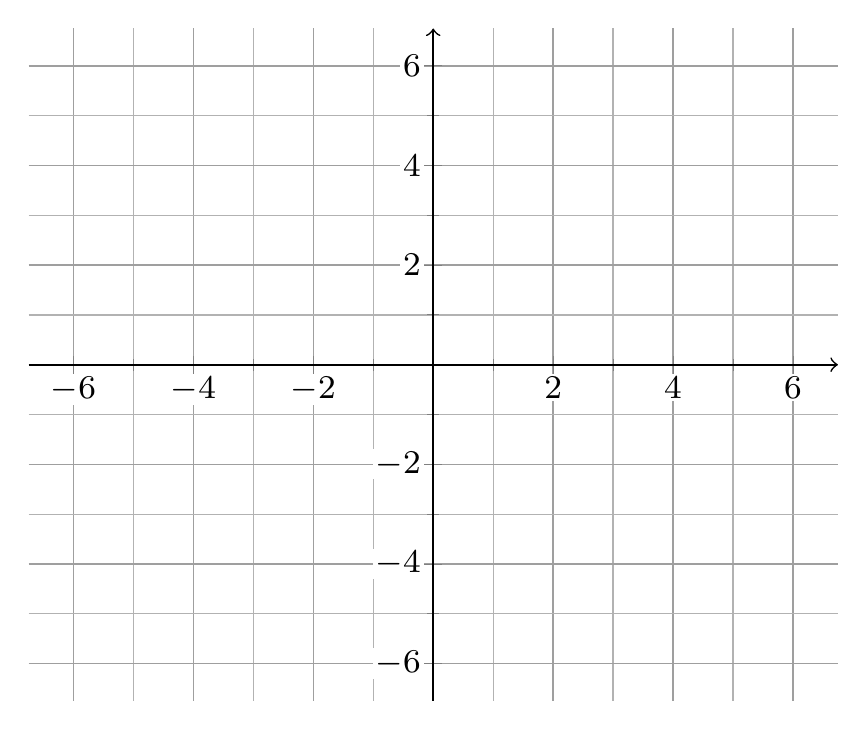
\begin{tikzpicture}[scale=1.5]
      \begin{axis}[
        grid=both, %major,minor
        grid style={line width=0.3pt, draw=gray!60},
        major grid style={line width=0.375pt, draw=gray!75},
        axis lines=center,
        axis line style={black,->},
        xmin=-6, xmax=6,
        ymin=-6, ymax=6,
        minor x tick num=1,
        minor y tick num=1,
        enlargelimits={abs=0.75},
        ticklabel style={font=\footnotesize,inner sep=0.65pt,fill=white,opacity=1.0, text opacity=1},
        every axis plot/.append style={line width=0.95pt, color=blue, samples=100}
        ]
      \end{axis}
    \end{tikzpicture}
  \end{center}
  \vspace*{\stretch{1}}
  \pagebreak

  \begin{ex*}
    Sketch the vector field $\mathbf F=\bracket{1-y^2,0}$ for $\abs{y}\leq 1$.
  \end{ex*}
  \vspace*{\stretch{1}}
  \begin{center}
    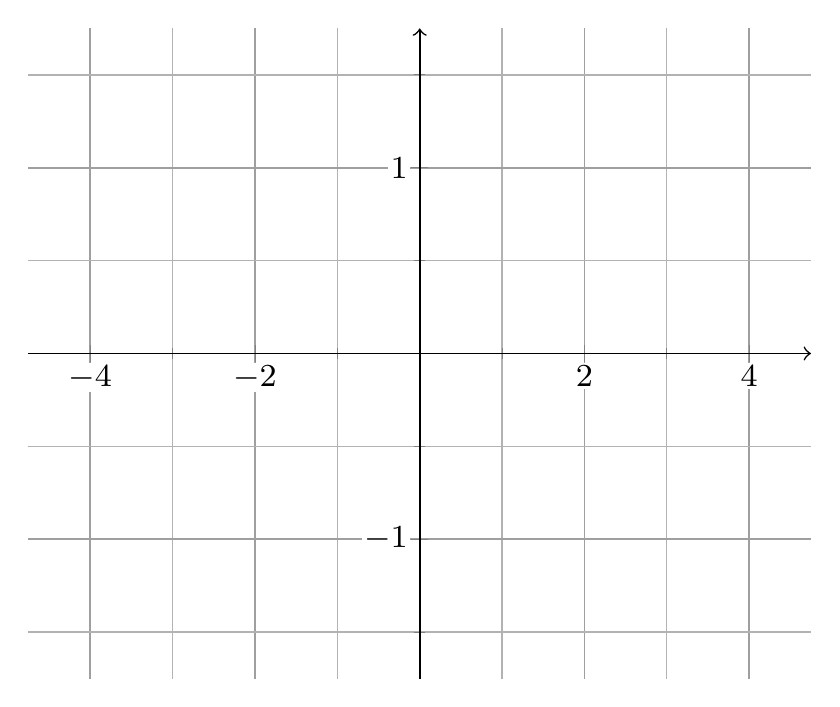
\begin{tikzpicture}[scale=1.45]
      \begin{axis}[
        grid=both, %major,minor
        grid style={line width=0.3pt, draw=gray!60},
        major grid style={line width=0.375pt, draw=gray!75},
        axis lines=center,
        axis line style={black,->},
        xmin=-4,   xmax=4,
        ymin=-1.0, ymax=1.0,
        minor x tick num=1,
        minor y tick num=1,
        enlargelimits={abs=0.75},
        ticklabel style={font=\footnotesize,inner sep=0.65pt,fill=white,opacity=1.0, text opacity=1},
        every axis plot/.append style={line width=0.95pt, color=blue, samples=100}
        ]
      \end{axis}
    \end{tikzpicture}
  \end{center}
  \vspace*{\stretch{1}}

  \begin{ex*}
    Sketch the vector field $\mathbf F=\bracket{-y,x}$.
  \end{ex*}
  \vspace*{\stretch{1}}
  \begin{center}
    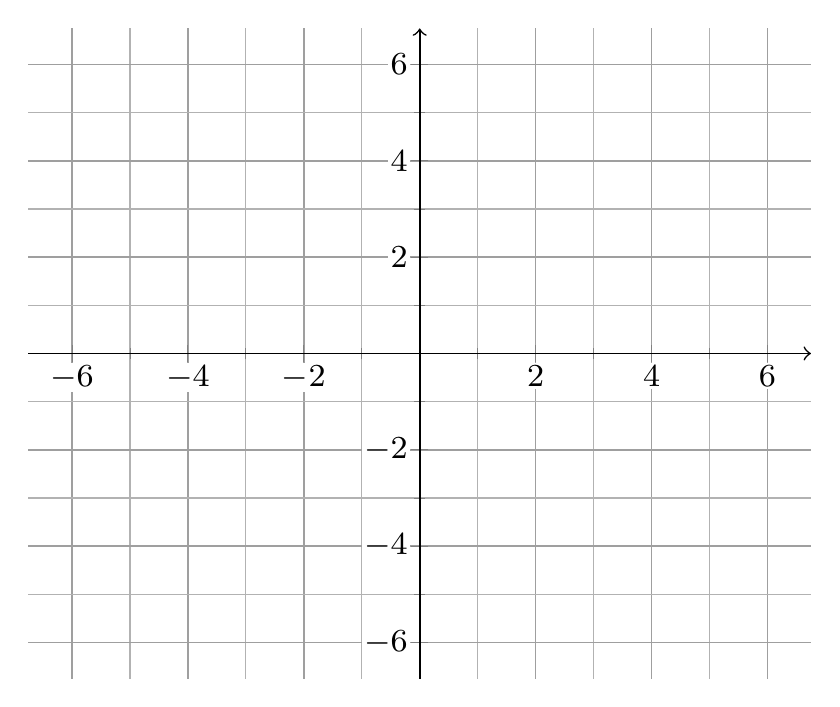
\begin{tikzpicture}[scale=1.45]
      \begin{axis}[
        grid=both, %major,minor
        grid style={line width=0.3pt, draw=gray!60},
        major grid style={line width=0.375pt, draw=gray!75},
        axis lines=center,
        axis line style={black,->},
        xmin=-6, xmax=6,
        ymin=-6, ymax=6,
        minor x tick num=1,
        minor y tick num=1,
        enlargelimits={abs=0.75},
        ticklabel style={font=\footnotesize,inner sep=0.65pt,fill=white,opacity=1.0, text opacity=1},
        every axis plot/.append style={line width=0.95pt, color=blue, samples=100}
        ]
      \end{axis}
    \end{tikzpicture}
  \end{center}
  \vspace*{\stretch{1}}
  \pagebreak

  \begin{defn*}[Radial Vector Fields in $\bbr^2$]
    Let $\vecr=\bracket{x,y}$. A vector field of the form $\mathbf F=f(x,y)\vecr$, where $f$ is a scalar valued function, is a \textbf{radial vector field}. Of specific interest are the radial vector fields
      \[\mathbf F(x,y)=\frac{\vecr}{\abs{\vecr}^p}=\frac{\bracket{x,y}}{\abs{\vecr}^p}=\frac{\vecr}{\abs{\vecr}}\,\frac{1}{\abs{\vecr}^{p-1}},\]
    where $p$ is a real number. At every point (expect the origin), the vectors of this field are directed outward from the origin with a magnitude of $\ds\abs{\mathbf F}= \frac{1}{\abs{\vecr}^{p-1}}$.
  \end{defn*}

  \begin{ex*}
    Let $C$ be the circle $x^2+y^2=a^2$, where $a>0$.
  \end{ex*}
  \begin{tasks}[after-item-skip=\stretch{1}, label=\alph*)](1)
    \task 
      Show that at each point of $C$, the radial vector field $\ds\mathbf F(x,y)=\frac{\vecr}{\abs{\vecr}}=\frac{\bracket{x,y}}{\sqrt{x^2+y^2}}$ is orthogonal to the line tangent to $C$ at that point.
    \task 
      Show that at each point of $C$, the rotation vector field $\ds\mathbf G(x,y)=\frac{\bracket{-y,x}}{\sqrt{x^2+y^2}}$ is parallel to the line tangent to $C$ at that point.
  \end{tasks}
  \vspace*{\stretch{1}}
  \pagebreak

  \begin{defn*}[Vector Fields and Radial Vector Fields in $\bbr^3$]
    Let $f$, $g$, and $h$ be defined on a region $D$ of $\bbr^3$. A \textbf{vector field} in $\bbr^3$ is a function $\mathbf F$ that assigns to each point in $D$ a vector $\bracket{f(x,y,z),\,g(x,y,z),\,h(x,y,z)}$. The vector field is written as
      \begin{align*}
        \mathbf F(x,y,z)&= \bracket{f(x,y,z),\,g(x,y,z),\,h(x,y,z)}\hspace*{15pt} \textnormal{ or}\\
        \mathbf F(x,y,z)&= f(x,y,z)\bfi+g(x,y,z)\bfj+h(x,y,z)\bfk.
      \end{align*}
    A vector field $\mathbf F=\bracket{f,g,h}$ is continuous or differentiable on a region $D$ of $\bbr^3$ if $f$, $g$, and $h$ are continuous or differentiable on $D$, respectively. Of particular importance are the \textbf{radial vector fields}
      \[\mathbf F(x,y,z)=\frac{\vecr}{\abs{\vecr}^p}=\frac{\bracket{x,y,z}}{\abs{\vecr}^p},\]
    where $p$ is a real number.
  \end{defn*}
  \begin{ex*}
    Sketch the vector field $\mathbf F(x,y,z)=\bracket{0,0,1-x^2-y^2}$, for $x^2+y^2\leq 1$.
  \end{ex*}
  \vspace*{\stretch{1}}
  \begin{center}
    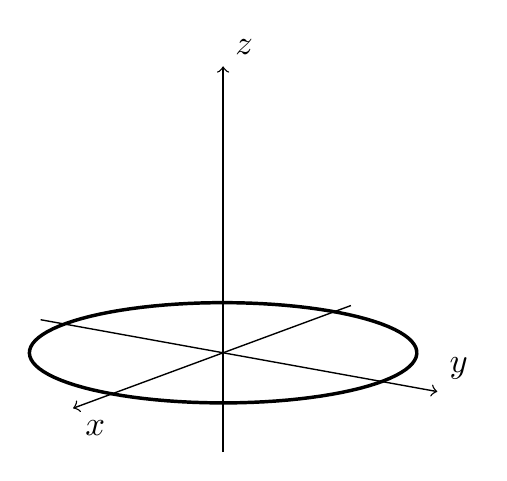
\begin{tikzpicture}[scale=1.25]
      \begin{axis}[
        axis lines=center,
        axis line style={black,->},
        axis equal,
        xmin=-1.15, xmax=1.35,  xmajorticks=false,
        ymin=-1.15, ymax=1.35,  ymajorticks=false,
        zmin=-0.25, zmax=1.25,  zmajorticks=false,
        ticklabel style={font=\normalsize,inner sep=0.5pt,fill=white,opacity=1.0, text opacity=1},
        xlabel=$x$, xlabel style={at={(ticklabel* cs:1)},anchor=north west},
        ylabel=$y$, ylabel style={at={(ticklabel* cs:1)},anchor=south west},
        zlabel=$z$, zlabel style={at={(ticklabel* cs:1)},anchor=south west},
        view={125}{15},
        ]
%        \addplot3[-] expression[domain=-1:1] {-sqrt(1-x^2)};
        \addplot3[domain=0:2*pi, samples=100, samples y=0, -, line width=1pt] ({cos(deg(x))},{sin(deg(x))},{0});
      \end{axis}
    \end{tikzpicture}
  \end{center}
  \vspace*{\stretch{1}}
  \pagebreak

  \begin{defn*}[Gradient Fields and Potential Functions]
    Let $\varphi$ be differentiable on a region of $\bbr^2$ or $\bbr^3$. The vector field $\mathbf =\grad \varphi$ is a \textbf{gradient field} and the function $\varphi$ is a \textbf{potential function} for $\mathbf F$.
  \end{defn*}

  \begin{ex*}
    Sketch and interpret the gradient field associated with the temperature function $T=200-x^2-y^2$ on the cirular plane $R=\set{(x,y): x^2+y^2\leq 25}$.
  \end{ex*}
  \vspace*{\stretch{1}}
  \begin{ex*}
    Sketch and interpret the gradient field associated with the velocity potential $\varphi=\tan\inv(xy)$.
  \end{ex*}
  \vspace*{\stretch{1}}
  \pagebreak
  
\end{document}
